\documentclass[a4paper]{jsarticle}
\usepackage[dvipdfmx]{graphicx}
\usepackage{amsmath}
\usepackage{bm}
\renewcommand{\thesection}{第\arabic{section}問}
\renewcommand{\thesubsection}{(\arabic{subsection})}
\renewcommand{\thesubsubsection}{(\alph{subsubsection})}
\begin{document}

\title{2012分野1}
\author{nakao}
\maketitle

\section{}
\subsection{}
\subsubsection{}
問題設定において$x$軸方向、$z$軸方向、回転モーメントのつりあいより、
図1のように点$B$における支点反力が得られる。
\begin{figure}[htb]
  \centering
  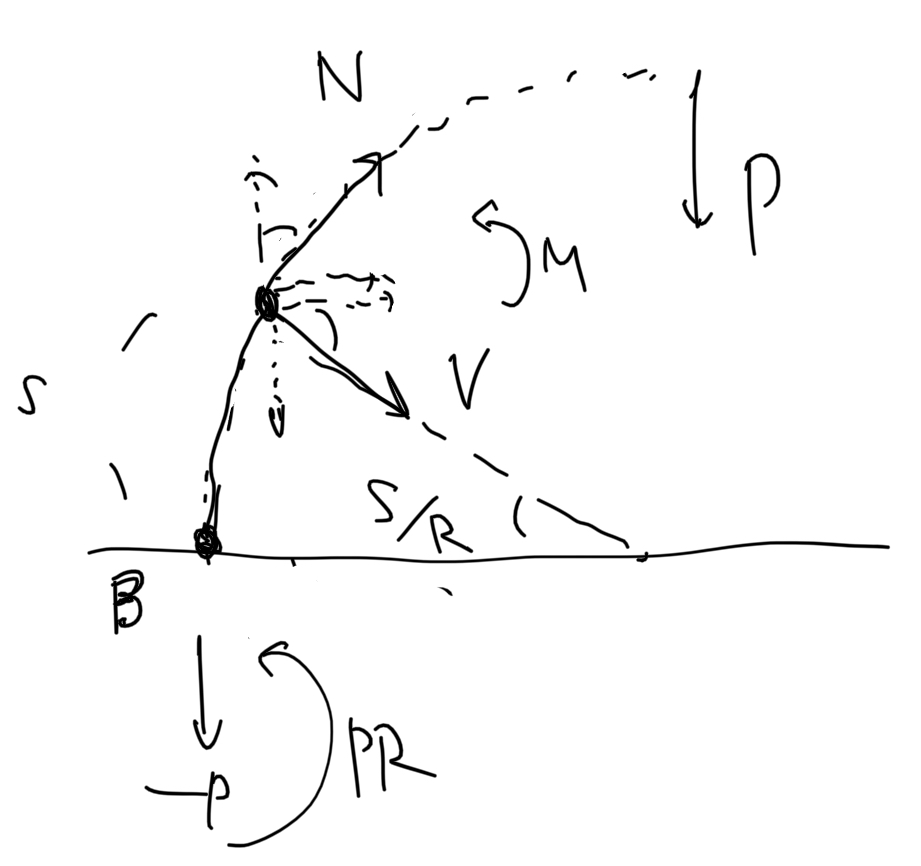
\includegraphics[width=0.3\hsize]{fig1.png}
  \caption{支点反力と内力}
\end{figure}
$s$座標が0からある$s$までの部分で力のつり合いを考えると、内力について
\begin{align}
  N \sin \frac{s}{R} + V \cos \frac{s}{R} &= 0 \\
  -N \cos \frac{s}{R} + V \sin \frac{s}{R} - P &= 0 \\
  M + P R - P R (1 - \cos \frac{s}{R}) &= 0
\end{align}
となる。これを解いて、
\begin{align}
  N &= -P \cos \frac{s}{R} \\
  V &= P \sin \frac{s}{R} \\
  M &= -P R \cos \frac{s}{R}
\end{align}
を得る。

\subsubsection{}
ベルヌーイ・オイラーの仮定より、
\begin{align}
  N &= E A \varepsilon \\
  M &= E I \lambda^{\prime}
\end{align}
が成り立つ。これより、
\begin{align}
  \varepsilon &= \frac{N}{E A} =
  -\frac{P}{E A} \cos \frac{s}{R} \\
  \lambda &= \lambda(s = 0)
  + \int_0^s \frac{M}{E I} \mathrm{d} s
  = -\frac{P R^2}{E I} \sin \frac{s}{R}
\end{align}
である。

\subsubsection{}
$s$軸に平行な方向の変位を$u_s$、垂直な方向の変位を$w_s$とする。
\begin{figure}
  \centering
  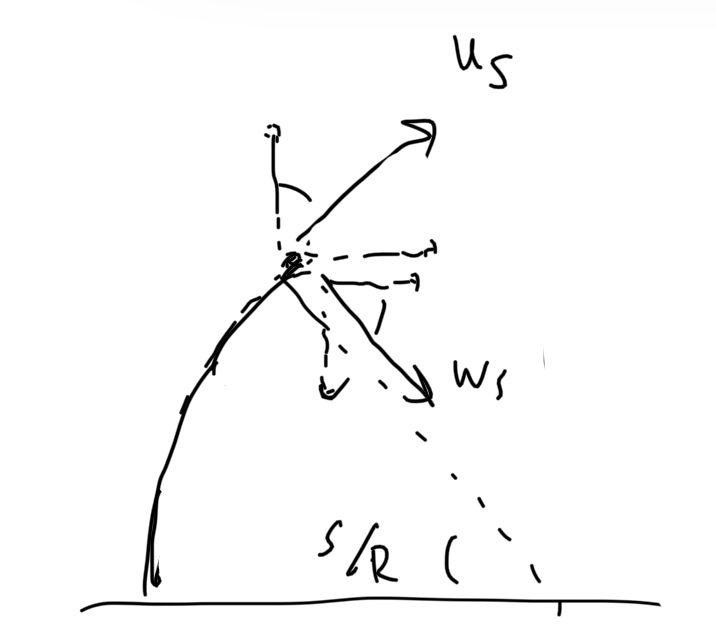
\includegraphics[width=0.3\hsize]{fig2.png}
  \caption{$u_s, w_s$の方向}
\end{figure}
$u, w, u_s, w_s$は図2のような関係にあり、
\begin{align}
  u &= u_s \sin \frac{s}{R} + w_s \cos \frac{s}{R} \\
  w &= -u_s \cos \frac{s}{R} + w_s \sin \frac{s}{R}
\end{align}
が成り立つ。式(11),(12)を$s$で微分し、
$\varepsilon = \frac{\mathrm{d} u_s}{\mathrm{d} s}, \lambda = -\frac{\mathrm{d} w_s}{\mathrm{d} s}$
を用いると、
\begin{align}
  \frac{\mathrm{d} u}{\mathrm{d} s}
  &= \varepsilon \sin \frac{s}{R} 
  - \lambda \cos \frac{s}{R} \\
  \frac{\mathrm{d} w}{\mathrm{d} s}
  &= -\varepsilon \cos \frac{s}{R} 
  - \lambda \sin \frac{s}{R}
\end{align}
であり、ここに式(9),(10)の分布を代入すると、
\begin{align}
  \frac{\mathrm{d} u}{\mathrm{d} s}
  &= -\frac{P}{E A} \cos \frac{s}{R} \sin \frac{s}{R}
  + \frac{P R^2}{E I} \cos \frac{s}{R} \sin \frac{s}{R} \\
  \frac{\mathrm{d} w}{\mathrm{d} s}
  &= \frac{P}{E A} \cos^2 \frac{s}{R} + \frac{P R^2}{E I} \sin^2 \frac{s}{R}
\end{align}
となる。

\subsubsection{}
式(15),(16)より、
\begin{align}
  u \left(s = \frac{\pi R}{2}\right) &= u(s = 0)
  + \int_0^{\frac{\pi R}{2}} \frac{\mathrm{d} u}{\mathrm{d} s} \mathrm{d} s
  = -\frac{P R}{2 E A} + \frac{P R^3}{2 E I}\\
  w \left(s = \frac{\pi R}{2}\right) &= w(s = 0)
  + \int_0^{\frac{\pi R}{2}} \frac{\mathrm{d} w}{\mathrm{d} s} \mathrm{d} s
  = \frac{\pi P R}{4 E A} + \frac{\pi P R^3}{4 E I}\\
\end{align}
を得る。

\subsection{}
$R = D/2$とする。
(1) a)と同様に支点反力を求め、内力とのつり合いを考えると、
\begin{align}
  N &= -Q \sin \frac{s}{R} \\
  V &= -Q \cos \frac{s}{R} \\
  M &= -Q R \sin \frac{s}{R}
\end{align}
を得る。ここで$s = \pi R / 2$に関する対称性より、
$\lambda(s = \pi R / 2) = 0$とすると、式(7),(8)より
\begin{align}
  \varepsilon &= \frac{N}{E A} =
  -\frac{Q}{E A} \sin \frac{s}{R} \\
  \lambda &= \lambda\left(s = \frac{\pi R}{2}\right)
  + \int_{\frac{\pi R}{2}}^s \frac{M}{E I} \mathrm{d} s
  = \frac{Q R^2}{E I} \cos \frac{s}{R}
\end{align}
となる。これらを式(13),(14)に代入すると、
\begin{align}
  \frac{\mathrm{d} u}{\mathrm{d} s}
  &= -\frac{Q}{E A} \sin^2 \frac{s}{R}
  - \frac{Q R^2}{E I} \cos^2 \frac{s}{R} \\
  \frac{\mathrm{d} w}{\mathrm{d} s}
  &= \frac{Q}{E A} \cos \frac{s}{R} \sin \frac{s}{R}
  - \frac{Q R^2}{E I} \cos \frac{s}{R} \sin \frac{s}{R}
\end{align}
を得る。したがって、
\begin{align}
  u \left(s = \frac{\pi R}{2}\right) &= u(s = 0)
  + \int_0^{\frac{\pi R}{2}} \frac{\mathrm{d} u}{\mathrm{d} s} \mathrm{d} s
  = -\frac{\pi Q R}{4 E A} - \frac{\pi Q R^3}{4 E I}\\
  w \left(s = \frac{\pi R}{2}\right) &= w(s = 0)
  + \int_0^{\frac{\pi R}{2}} \frac{\mathrm{d} w}{\mathrm{d} s} \mathrm{d} s
  = \frac{Q R}{2 E A} - \frac{Q R^3}{2 E I}
\end{align}
である。$R = D/2$を代入すると、
\begin{align}
  u \left(s = \frac{\pi R}{2}\right)
  &= -\frac{\pi Q D}{8 E A} - \frac{\pi Q D^3}{32 E I} \\
  w \left(s = \frac{\pi R}{2}\right)
  &= \frac{Q D}{4 E A} - \frac{Q D^3}{16 E I}
\end{align}
を得る。

\section{}
\subsection{}
運動方程式は、
\begin{equation}
  \begin{aligned}
    m \ddot{x}_1 + k x_1 + k (x_1 - x_2) &= -m \ddot{z} \\
    m \ddot{x}_2 + k (x_2 - x_1) &= -m \ddot{z}
  \end{aligned}
\end{equation}
であり、これを行列表示すると、
\begin{equation}
  \begin{pmatrix}
    m & 0 \\
    0 & m
  \end{pmatrix}
  \begin{pmatrix}
    \ddot{x}_1 \\
    \ddot{x}_2
  \end{pmatrix} +
  \begin{pmatrix}
    2k & -k \\
    -k & k
  \end{pmatrix}
  \begin{pmatrix}
    x_1 \\ x_2
  \end{pmatrix} =
  \begin{pmatrix}
    -m \ddot{z} \\
    -m \ddot{z}
  \end{pmatrix}
\end{equation}
である。

\subsection{}
行列$M,K$を
\begin{equation}
  M =
  \begin{pmatrix}
    m & 0 \\
    0 & m
  \end{pmatrix},\quad
  K =
  \begin{pmatrix}
    2k & -k \\
    -k & k
  \end{pmatrix}
\end{equation}
と定義すると、固有振動数$\omega$と固有モード$\boldsymbol{\phi}$について、
\begin{equation}
  (K - \omega^2 M) \boldsymbol{\phi} = \boldsymbol{0}
\end{equation}
が成り立つ。$\boldsymbol{\phi} = 0$となる解が存在するには、
\begin{equation}
  \det (K - \omega^2 M) = 0
\end{equation}
が必要である。式(35)を解くと、
\begin{equation}
  \omega = \sqrt{\frac{3 \pm \sqrt{5}}{2}} \omega_0
\end{equation}
となる。ここで、$\omega_0 = \sqrt{k / m}$である。\par
$\omega = \sqrt{\frac{3 - \sqrt{5}}{2}} \omega_0$のとき、
式(34)を解くと、
\begin{equation}
  \boldsymbol{\phi} \propto
  \begin{pmatrix}
    1 \\
    \frac{1 + \sqrt{5}}{2}
  \end{pmatrix}
\end{equation}
である。これを1次モードとすると、
\begin{equation}
  \omega_1 = \sqrt{\frac{3 - \sqrt{5}}{2}} \omega_0 \quad
  \boldsymbol{\phi}_1 =
  \begin{pmatrix}
    1 \\
    \frac{1 + \sqrt{5}}{2}
  \end{pmatrix}
\end{equation}
である。\par
$\omega = \sqrt{\frac{3 + \sqrt{5}}{2}} \omega_0$のとき、
式(34)を解くと、
\begin{equation}
  \boldsymbol{\phi} \propto
  \begin{pmatrix}
    1 \\
    \frac{1 - \sqrt{5}}{2}
  \end{pmatrix}
\end{equation}
である。これを2次モードとすると、
\begin{equation}
  \omega_2 = \sqrt{\frac{3 + \sqrt{5}}{2}} \omega_0 \quad
  \boldsymbol{\phi}_2 =
  \begin{pmatrix}
    1 \\
    \frac{1 - \sqrt{5}}{2}
  \end{pmatrix}
\end{equation}
である。\par

\subsection{}
ベクトル$\boldsymbol{P}, \boldsymbol{x}$を
\begin{equation}
  \boldsymbol{P} =
  \begin{pmatrix}
    -m \ddot{z} \\
    -m \ddot{z}
  \end{pmatrix} =
  \begin{pmatrix}
    m z_0 \omega^2 \sin \omega_t \\
    m z_0 \omega^2 \sin \omega_t
  \end{pmatrix}, \quad
  \boldsymbol{x} =
  \begin{pmatrix}
    x_1 \\ x_2
  \end{pmatrix}
\end{equation}
とすると、運動方程式は、
\begin{equation}
  M \ddot{\boldsymbol{x}} + K \boldsymbol{x} = \boldsymbol{P}
\end{equation}
と表せる。
$\boldsymbol{x}$を固有振動の重ね合わせとして、
スカラー$q_1, q_2$を用いて
\begin{equation}
  \boldsymbol{x}
  = q_1 \boldsymbol{\phi}_1 + q_2 \boldsymbol{\phi}_2
\end{equation}
と表すと、固有モードの直交性より、
\begin{equation}
  \begin{aligned}
    \boldsymbol{\phi}_1^T M \boldsymbol{\phi}_1 \ddot{q}_1
    + \boldsymbol{\phi}_1^T K \boldsymbol{\phi}_1 \ddot{q}_1
    &= \boldsymbol{\phi}_1^T \boldsymbol{P} \\
    \boldsymbol{\phi}_2^T M \boldsymbol{\phi}_2 \ddot{q}_2
    + \boldsymbol{\phi}_2^T K \boldsymbol{\phi}_2 \ddot{q}_2
    &= \boldsymbol{\phi}_2^T \boldsymbol{P}
  \end{aligned}
\end{equation}
が成り立つ。これを計算すると、
\begin{equation}
  \begin{aligned}
    \frac{5 + \sqrt{5}}{2} m \ddot{q}_1
    + \frac{5 - \sqrt{5}}{2} k q_1
    &= \frac{3 + \sqrt{5}}{2} m z_0 \omega^2 \sin \omega t \\
    \frac{5 - \sqrt{5}}{2} m \ddot{q}_2
    + \frac{5 + \sqrt{5}}{2} k q_2
    &= \frac{3 - \sqrt{5}}{2} m z_0 \omega^2 \sin \omega t \\
  \end{aligned}
\end{equation}
を得る。この強制振動の方程式に対する定常解は、
\begin{equation}
  \begin{aligned}
    q_1 &= \frac{\frac{3 + \sqrt{5}}{2} m z_0 \omega^2}{\frac{5 - \sqrt{5}}{2} k}
    \frac{1}{1 - \left(\frac{\omega}{\omega_1}\right)^2} \sin \omega t
    = \frac{4 z_0 \omega^2}{(5 - \sqrt{5})\{(3 - \sqrt{5}) \omega_0^2 - 2 \omega^2\}} \\
    q_2 &= \frac{\frac{3 - \sqrt{5}}{2} m z_0 \omega^2}{\frac{5 + \sqrt{5}}{2} k}
    \frac{1}{1 - \left(\frac{\omega}{\omega_2}\right)^2} \sin \omega t
    = \frac{4 z_0 \omega^2}{(5 + \sqrt{5})\{(3 + \sqrt{5}) \omega_0^2 - 2 \omega^2\}}
  \end{aligned}
\end{equation}
と求められる。これを式(43)に代入すると、
$\boldsymbol{x}$の定常応答は、
\begin{equation}
  \boldsymbol{x} = 
  \begin{pmatrix}
    x_1 \\
    x_2 \\
  \end{pmatrix} =
  \frac{\omega^2  z0}{\omega^4 - 3 \omega^2 \omega_0^2 + \omega_0^4}
  \begin{pmatrix}
    2 \omega_0^2 - \omega^2 \\ 
    3 \omega_0^2 - \omega^2 \\
  \end{pmatrix}
  \sin \omega t
\end{equation}
と求められる。$x_1 = 0$または$x_2 = 0$が任意の時間で成り立つには、
\begin{equation}
  \omega = \sqrt{2} \omega_0, \sqrt{3} \omega
\end{equation}
であればよい。

\subsection{}
式(47)より、
\begin{equation}
  \begin{aligned}
    X_1(\omega) &= \left|\frac{\omega^2 (2 \omega_0^2 - \omega^2) z0}{\omega^4 - 3 \omega^2 \omega_0^2 + \omega_0^4}\right| \\
    X_2(\omega) &= \left|\frac{\omega^2 (3 \omega_0^2 - \omega^2) z0}{\omega^4 - 3 \omega^2 \omega_0^2 + \omega_0^4}\right| \\
  \end{aligned}
\end{equation}
である。これを固有振動数$\omega = \omega_1, \omega2$、
零点$\omega = \sqrt{2} \omega_0, \sqrt{3} \omega$、
無限大$\omega \to \infty$について求めると、
\begin{align}
  \left(X_1(\omega_1), X_2(\omega_1)\right) &= (\infty, \infty) \\
  \left(X_1(\omega_2), X_2(\omega_2)\right) &= (\infty, \infty) \\
  \left(X_1(\sqrt{2} \omega_0), X_2(\sqrt{2} \omega_0)\right) &= (0, 2 z_0) \\
  \left(X_1(\sqrt{3} \omega_0), X_2(\sqrt{3} \omega_0)\right) &= (3 z_0, 0) \\
  \left(X_1(\infty), X_2(\infty)\right) &= (z_0, z_0)
\end{align}
である。任意の$\omega > 0$に対して
$X_1(\omega), X_2(\omega)$を図示すると、
図3,4のようになる。
\begin{figure}
  \begin{minipage}{0.5\hsize}
    \centering
    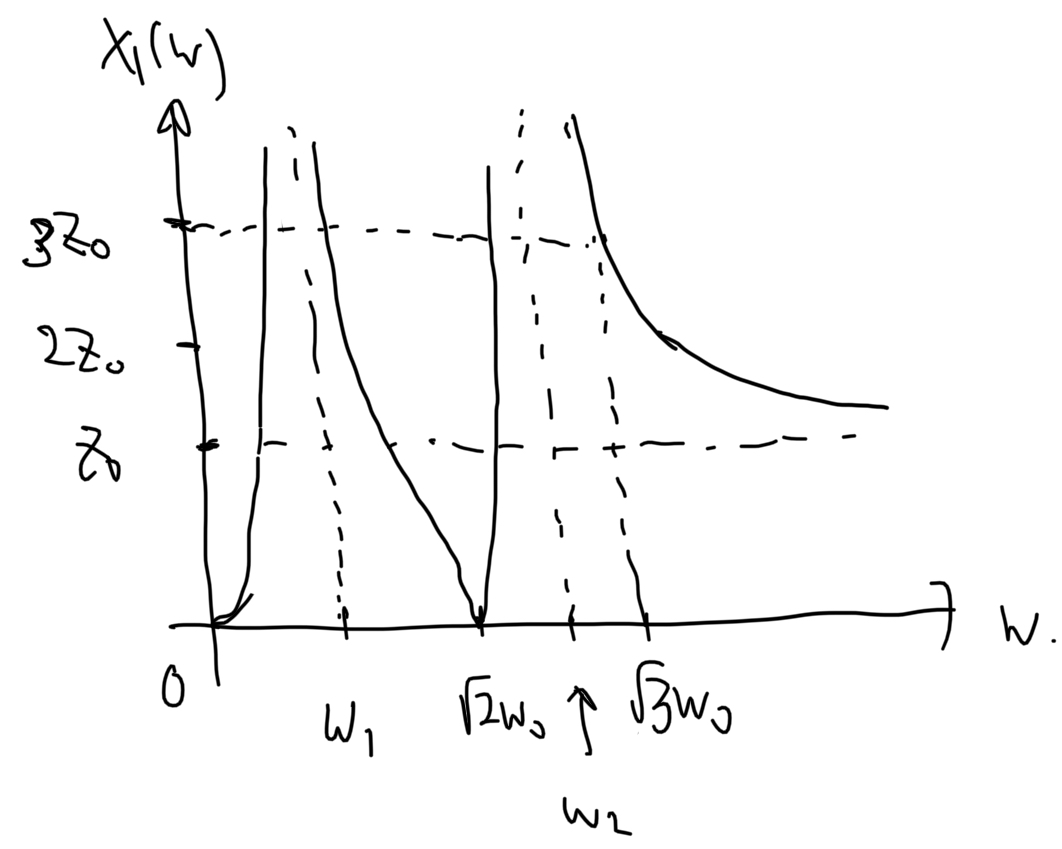
\includegraphics[width=\hsize]{fig3.png}
    \caption{$X_1$の分布}
  \end{minipage}
  \begin{minipage}{0.5\hsize}
    \centering
    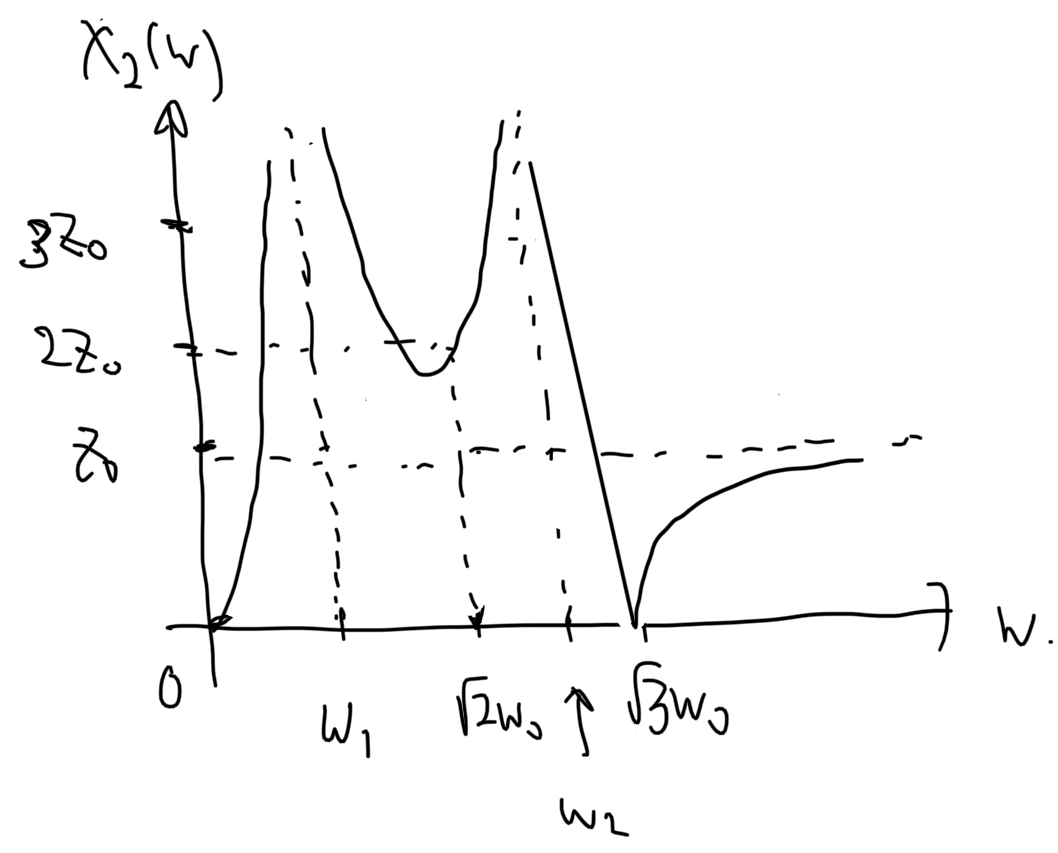
\includegraphics[width=\hsize]{fig4.png}
    \caption{$X_2$の分布}
  \end{minipage}
\end{figure}

\subsection{}
質量が多数の層になって分布しているときには、
特定の層で応答が大きくなる外力の振動数において、
他の層での応答が小さくなる場合がある。
複数の振動モードを検討して、それぞれの層において厳しくなるような外力を別々に設定する必要がある。
\end{document}
